\section{Requisiti Soddisfatti}

\begin{table}[!htbp]
\rowcolors{2}{gray!25}{white}
\renewcommand{\arraystretch}{1.5}
\begin{tabular}[t]{ m{0.15\textwidth}<{\centering}  m{0.3\textwidth}<{\centering} }
	\rowcolor{darkblue}
	\textcolor{white}{\textbf{Fonte}} &\textcolor{white}{\textbf{Requisiti}}\\ 

	R1FW1 & \So \\	
	 
	R1FW2 & \So \\	

	R2FW3 & \So \\	
	 
	R1FE1 & \So \\	
	 
	R1FE2 & \So \\	
	 
	R1FE3 & \So \\	

	R1FE4 & \So \\	
	
	R1FE5 & \So \\
	 
	R1FE6 & \So \\	 
	 
	R1FE7 & \So \\	

	R1FW4 & \So \\ 
	 
	R1FW4.1& \Ns \\	
	 
	R1FE8 & \Ns \\	
	 
	R1FW4.2 & \Ns \\		 

	R1FE9 & \Ns \\		
	 
	R3FW4.3 & \So \\				
	 
	R3FE15 & \So \\			
	  	 	 	
	R1FW5 & \So \\		
	
	R2FE10 & \Ns \\
	
	R2FE11 & \Ns \\
	 
	R2FE12 & \Ns \\			
	 
	R1FW7 & \So \\	
	
	R1FW7.1 & \So \\

	R1FW7.2 & \So \\
	
	R2FW7.3 & \So \\
	
	R2FW7.4 & \So \\		
	
	R1FW8 & \Ns \\		
	
	R2FE13 & \Ns \\	
	 
	R1FW8.1 & \Ns \\	
	
	R2FW8.2 & \Ns \\

\end{tabular}
\begin{tabular}[t]{ m{0.15\textwidth}<{\centering}  m{0.3\textwidth}<{\centering} }
	\rowcolor{darkblue}
	\textcolor{white}{\textbf{Fonte}} &\textcolor{white}{\textbf{Requisiti}}\\ 	
	 
	R2FW8.3 & \Ns \\	
	 
	R2FW8.4 & \Ns \\	 
	 
	R1FW8.5 & \Ns \\	 
	 
	R3FW9 & \Ns \\	
	 
	R3FW9.1& \Ns \\	 
	 
	R3FW9.2& \Ns \\	  
	 
	R1FW10 & \So \\	 
	 
	R2FE14& \So \\	 
	 	 
	R1FW11& \So \\	 	
	
	R2FW11.1 & \So \\
 	
	R2FW11.2 & \So \\
 	
	R2FW11.3 & \So \\
 
	R2FW11.4 & \Ns \\
	
	R1FW11.1.1 & \So \\
		
	R2FW11.1.2 & \So \\
		
	R2FW11.1.3 & \So \\
	
	R3FW11.1.4& \Ns \\
	
	R2FW11.1.5& \Ns \\
	
	R2FW11.1.6 & \So \\
	
	R1FW11.2.1 & \So \\

	R1FW11.2.2 & \So \\	
	
	R1FW11.2.3 & \So \\
	
	R1FW11.2.4 & \So \\
	
	R2FW11.3.1 & \So \\
	
	R2FW11.3.2 & \So \\
	
	R2FW11.3.3 & \So \\

	R2FW12& \Ns \\

	R2FW13 & \Ns \\

	R3F1 & \Ns \\


\end{tabular}
\caption{Tabella soddisfacimento requisiti}
\end{table}

\newpage

\subsection{Grafici relativi al soddisfacimento dei requisiti}

\subsubsection{Requisiti soddisfatti vs. non soddisfatti}

Il seguente grafico a torta mostra la percentuale di requisiti del nostro prodotto che sono stati soddisfatti, ossia 36 requisiti soddisfatti (il 61\%) su un totale di 59 (i requisiti rimasti da soddisfare sono 23).

\begin{figure}[H]
    \centering
    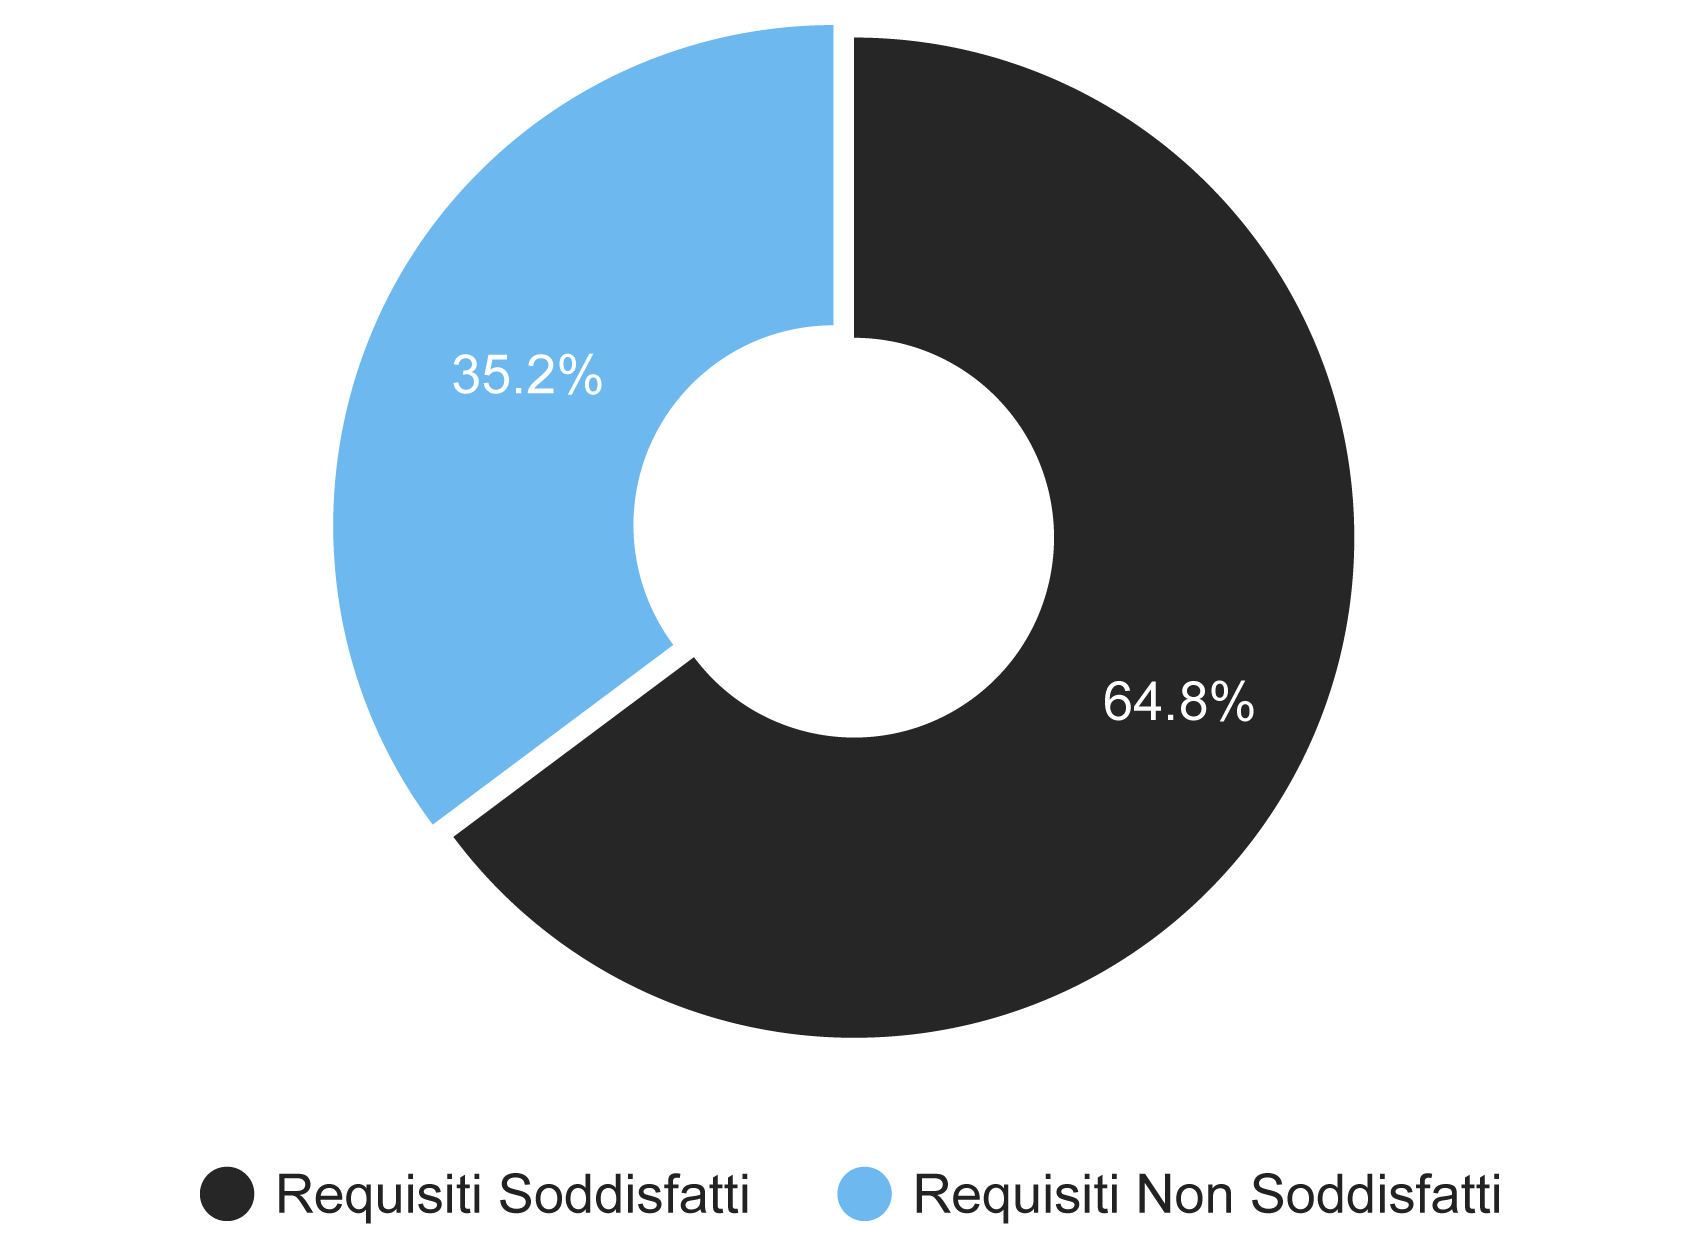
\includegraphics[scale=0.7]{Contenuto/Immagini/ReqSoddisfatti.png}
    \caption{Percentuale Requisiti Soddisfatti vs. Requisiti Non Soddisfatti}
\end{figure}

\subsubsection{Requisiti Obbligatori Soddisfatti}

Inizialmente, erano stati definiti 28 requisiti funzionali obbligatori da soddisfare per il nostro prodotto. Allo stato attuale ne sono stati soddisfatti 21 (il 75\%) e ne rimangono ancora da soddisfare 7.

\begin{figure}[H]
    \centering
    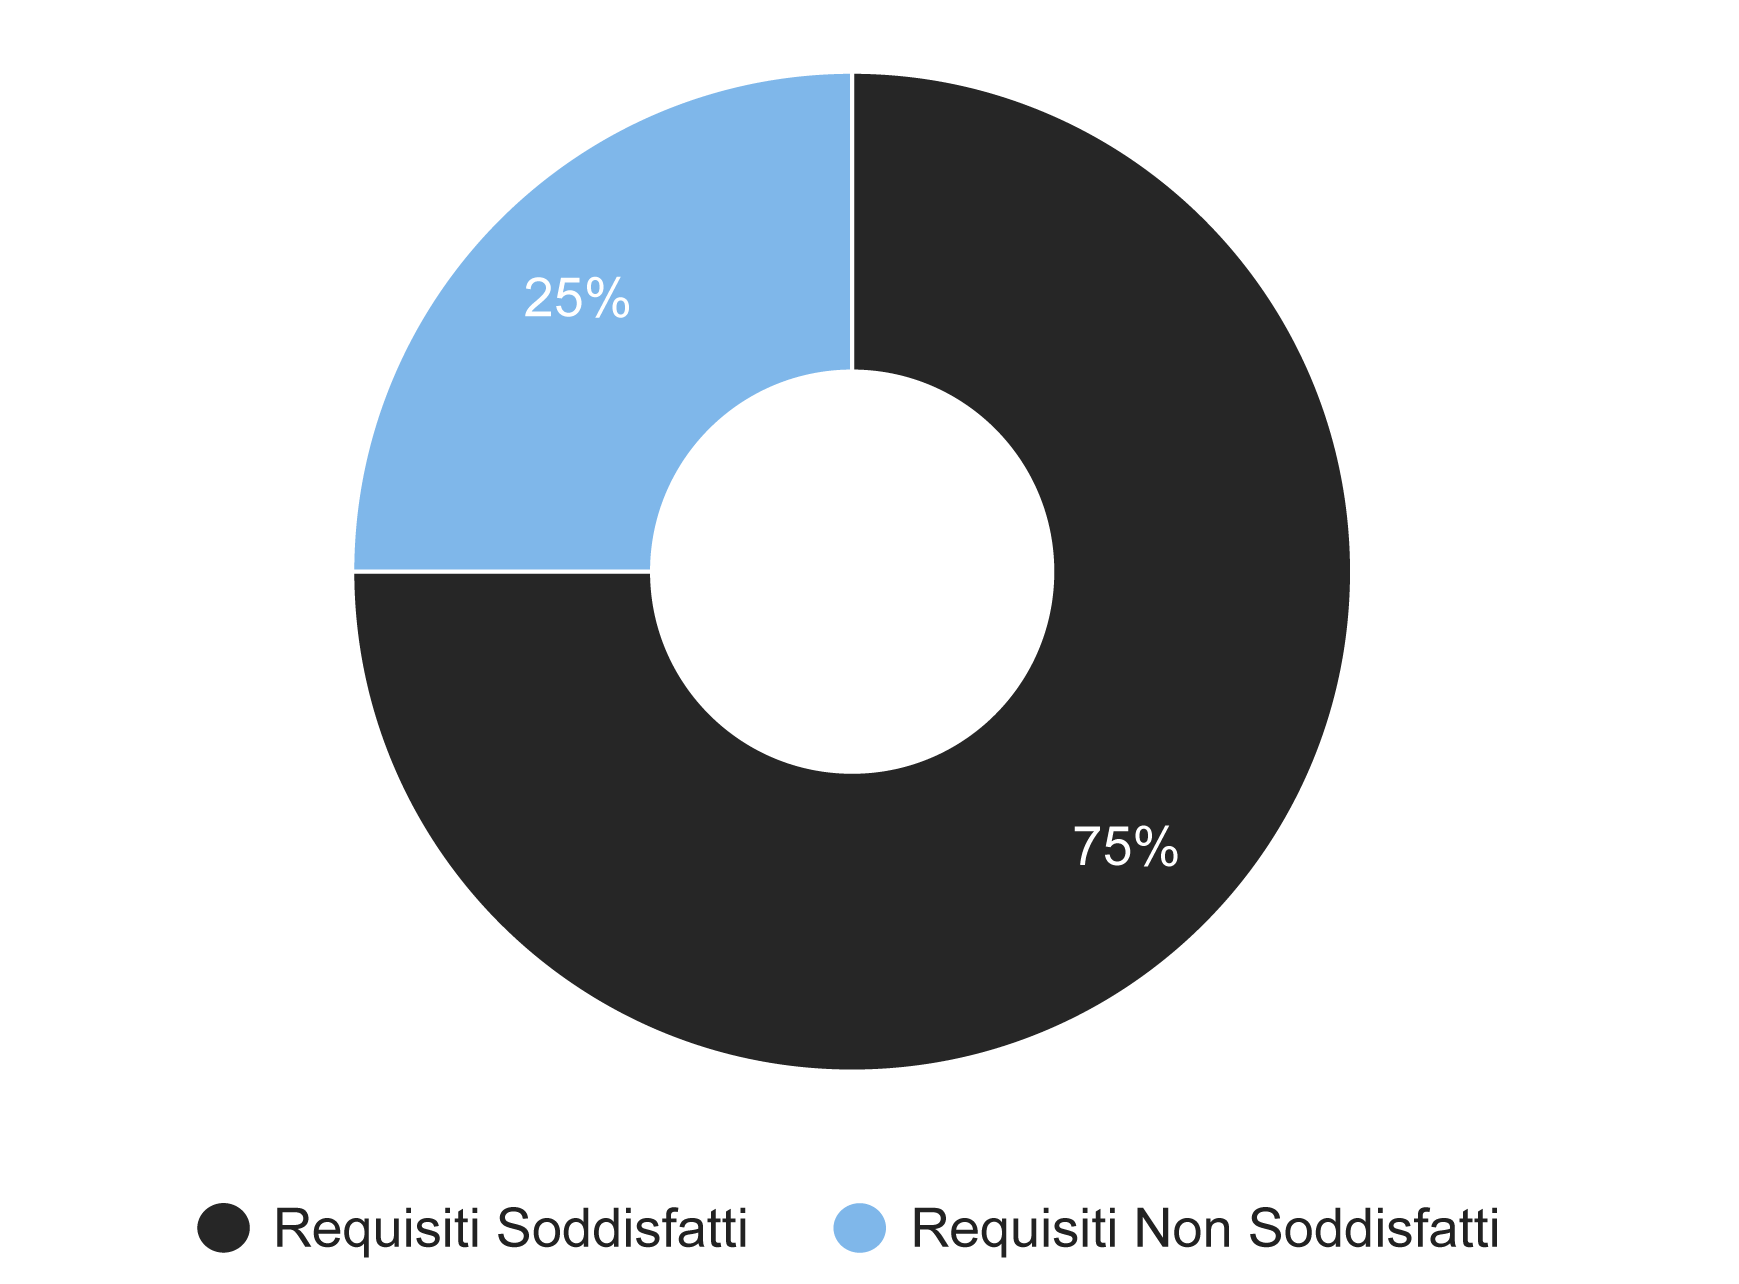
\includegraphics[scale=0.7]{Contenuto/Immagini/ReqObbligatoriSodd.png}
    \caption{Percentuale Requisiti Obbligatori Soddisfatti vs. Non Soddisfatti}
\end{figure}